\chapter{Описание алгоритма}
\label{cha:ch_2}

В данной главе будет описано обратимое и устойчивое к искажениям преобразование для построения спектрограммы из аудиосигнала.
Оно строится на основе операции многоканальной 1D свертки с заранее сформированным ядром, а также некоторой постобработки.

\section{Теоретическое обоснование алгоритма}
Напомним формулу 1D свертки. Пусть на входе есть двумерный массив данных $x: [L_{in} \times  C_{in}]$ 
и ядро свертки в виде массива $K: [C_{out} \times N \times C_{in}]$. Также задан шаг свертки $s$.
Тогда результат операции $y: [L_{out} \times C_{out}]$ рассчитывается по следующей формуле:
\begin{equation}
	y[i, c_{out}] = \sum_{j=0}^{N-1} \sum_{c_{in}=0}^{C_{in}-1} x[i \cdot s + j, c_{in}] \cdot K[c_{out}, j, c_{in}]
\end{equation}
\[i \in [0, L_{out}), \quad c_{out} \in [0, C_{out})\]
\[L_{out} = \lfloor(L_{in} - N) / s\rfloor + 1\]

\begin{figure}
  \centering
  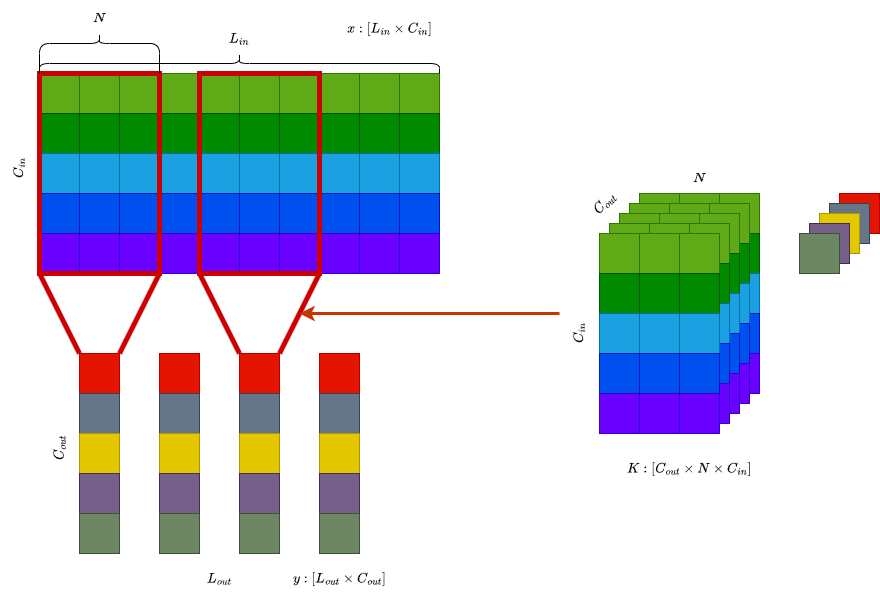
\includegraphics[width=0.9\linewidth]{figures/conv1d_drawio}
  \caption{Иллюстрации операции 1D свертки}
  \label{fig:conv1d_drawio}
\end{figure}

Каждый вектор $y_i: [1 \times C_{out}]$ можно рассматривать как матричное умножение вырезанного окна $x_i: [1 \times (N \cdot C_{in})]$ на матрицу $K^T: [(N \cdot C_{in}) \times C_{out}]$.

В случае, когда входным массивом является аудиосигнал, количество входных каналов $C_{in} = 1$, и можно несколько упростить формулу. 
\[x: [L_{in}], \quad K: [C_{out} \times N]\]
\begin{equation}
	y[i, c_{out}] = \sum_{j=0}^{N-1} x[i \cdot s + j] \cdot K[c_{out}, j]
\end{equation}


\textbf{Дискретное оконное преобразование Фурье (STFT)} можно посчитать через 1D свертку, если сформировать ядро $K_{\mathrm{stft}}: [N \times N]$ следующим образом:
\begin{equation}
	K_{\mathrm{stft}}[k, n] = e^{-i\pi \frac{(n - N/2) \cdot k}{N}} * w[n]
\end{equation}

\textbf{Дискретное вейвлет-преобразование (DWT)} на основе вейвлета Морле можно построить с помощью свертки с таким ядром:
\begin{equation}
	K_{\mathrm{dwt}}[k, n] = \psi^* \left(\frac{n - N/2}{a_0^k}\right)
\end{equation}
\[\psi(t) = e^{i\pi t} * e^{-\left(\frac{\pi t}{2\sigma}\right)^2}, \quad   a_0 \in (1, \infty)\]

На рисунке \ref{fig:stft_kernel} изображены ядра сверток для указанных преобразований, а также для преобразования, которое будет описано в данной работе.

\begin{figure}
  \centering
  \subfigure{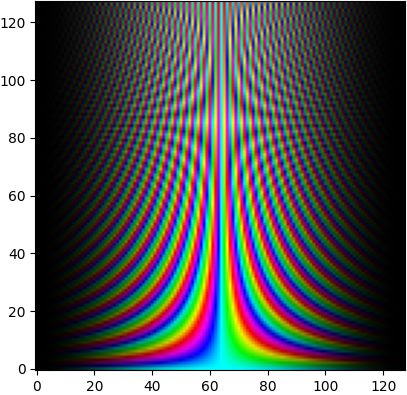
\includegraphics[width=0.3\textwidth]{figures/stft_kernel}} 
  \subfigure{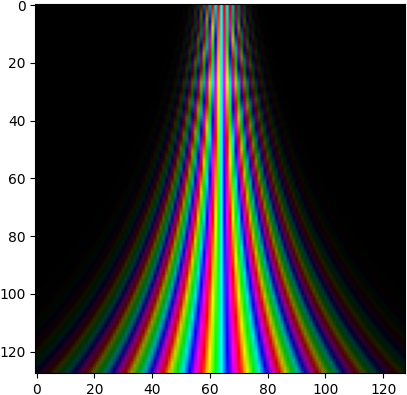
\includegraphics[width=0.3\textwidth]{figures/dwt_kernel}} 
  \subfigure{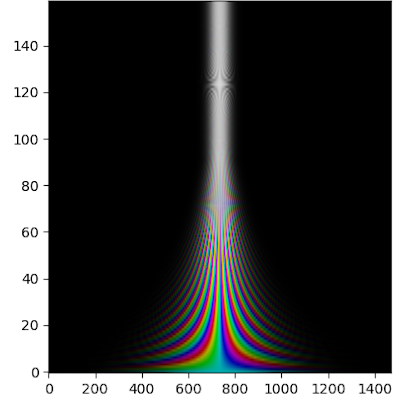
\includegraphics[width=0.3\textwidth]{figures/my_kernel}} 
  \caption{Ядро 1D свертки для STFT (1), вейвлет преобразования (2) и предлагаемого в работе преобразования (3)}
  \label{fig:stft_kernel}
\end{figure}


Теперь опишем процесс восстановления сигнала с помощью свертки, и при каких условиях он возможен.

Для начала рассмотрим преобразование, дискретное по частотам, но непрерывное по времени, 
представляющее собой свертку сигнала $x(t)$ с вейвлетом $\psi_m(t) = \Delta f_m \cdot e^{2\pi i f_m t} \cdot w(t\,\Delta f_m)$.
Здесь $\Delta f_m$ - расстояние между соседними частотами на выбранной шкале частот. $w(t)$ - оконная функция, она должна быть симметричной.

\begin{equation}
  S_m(t)=\int \limits _{-\infty}^{+\infty}x(\tau)\,\psi_m(t - \tau)\,d\tau = \{x * \psi_m\}(t)
  \label{eq:conv_x_psi}
\end{equation}

Здесь и далее, запись $\{u*v\}(t)$ обозначает свертку в математическом смысле, которая определяется следующим образом:

\begin{equation}
  \{u*v\}(t)\triangleq \int \limits_{-\infty }^{\infty }u(\tau )v(t-\tau )\,d\tau = \int \limits_{-\infty }^{\infty }u(t-\tau )v(\tau )\,d\tau
\end{equation}

Полученная в равенстве \ref{eq:conv_x_psi} функция $S_m(t)$ представляет собой сигнал, ограниченный некоторой полосой частот, 
определяемой центральной частотой $f_m$ и спектральной шириной окна $\Delta f_m$.
Если посчитать спектр сигнала $S_m(t)$ с помощью преобразования Фурье, то, согласно теореме о свертке \cite{conv_theorem}, 
получим произведение спектра исходного сигнала $\mathcal{F}\{x(t)\}$ и спектра вейвлета $\mathcal{F}\{\psi_m(t)\}$.
Спектр вейвлета представляет собой спектр оконной функции, центр которого сдвинут к частоте $f_m$.

\begin{equation}
  \mathcal{F}\{S_m\}(f) = \mathcal{F}\{x\}(f) \cdot \mathcal{F}\{\psi_m\}(f)
\end{equation}

Если произвести снова свертку $S_m(t)$ с вейвлетом $\psi_m(t)$ в качестве этапа восстановления и посчитать спектр полученного сигнала, получим:

\begin{equation}
  \tilde{x}_m(t) = \{S_m * \psi_m\}(t) = \int \limits _{-\infty}^{+\infty} S_m(\tau)\,\psi_m(t - \tau)\,d\tau
\end{equation}
\begin{equation}
  \mathcal{F}\{\tilde{x}_m\} = \mathcal{F}\{S_m\} \cdot \mathcal{F}\{\psi_m\} = \mathcal{F}\{x\} \cdot (\mathcal{F}\{\psi_m\})^2
\end{equation}

Заметим, что спектр вейвлета является действительным в силу его симметричности $\psi(-t) = \psi^{*}(t)$, и равен спектру оконной функции, сдвинутым к центральной частоте $f_m$:
\begin{equation}
  \mathcal{F}\{\psi_m\}(f) = \Delta f_m \cdot \mathcal{F}\{w(t\,\Delta f_m)\}(f - f_m) = \mathcal{F}\{w(t)\}\left(\frac{f - f_m}{\Delta f_m}\right)
\end{equation}

При достаточно плотном перекрытии окон на оси частот, спектр исходного сигнала $\mathcal{F}\{x\}$ можно представить как взвешенную сумму:
\begin{equation}
  \mathcal{F}\{x\} = \frac{
    \sum \limits_m \mathcal{F}\{x\} \cdot (\mathcal{F}\{\psi_m\})^2
  }{
    \sum \limits_m (\mathcal{F}\{\psi_m\})^2
  } = 
  \frac{
    \sum \limits_m \mathcal{F}\{\tilde{x}_m\}(f)
  }{
    \sum \limits_m (\mathcal{F}\{\psi_m\})^2(f)
  }
  \label{eq:back_weighted_sum}
\end{equation}

Если записать спектр каждого вейвлета как сдвинутый и растянутый спектр окна, получим следующее равенство:

\begin{equation}
  \mathcal{F}\{x\} = 
  \frac{
    \sum \limits_m \mathcal{F}\{\tilde{x}_m\}(f)
  }{
    \sum \limits_m (\mathcal{F}\{w(t)\})^2 \left(\frac{f - f_m}{\Delta f_m}\right)
  }
  \label{eq:wavelets_back_spec}
\end{equation}


Для получения обратной формулы покажем, что при достаточно плотном перекрытии окон на оси частот
знаменатель последней дроби является константой на любой частоте $f$ и рассчитаем его.

\textbf{Утверждение 1}. Рассмотрим сумму в знаменателе как интеграл по частотам.
Если ввести функцию шкалы частот $f(m)$ и рассмотреть рассточние между частотами $\Delta f_m$ как производную этой функции $\frac{df}{dm}$,
данная сумма будет стремиться к интергалу следующего вида, который равен $w(0)$:
\begin{equation}
\sum \limits_m \mathcal{F}\{w(t)\} \left(\frac{f_0 - f_m}{\Delta f_m}\right) 
  \xrightarrow[M \to \infty]{} 
\int \limits_{-\infty}^\infty \mathcal{F}\{w(t)\} \left(\frac{f_0 - f(m)}{\frac{df}{dm}}\right) \, dm
  = I
\end{equation}
\[
I = w(0) + \varepsilon
\]

\textbf{Доказательство} для значения интеграла:

Разложив $f(m)$ по формуле Тейлора до первой производной, получим:
\begin{equation}
  f_0 - f(m) = (m_0 - m) \cdot \frac{df}{dm} + \frac{1}{2} \frac{d^2f(\theta)}{dm^2} (m - m_0)^2
\end{equation}

Если в пределах ширины окна функция $f(m)$ почти линейна, последний член пренебрежимо мал по сравнению с первым. 
Всегда можно отмасштабировать оконную функцию так, чтобы на каждой частоте в пределах ширины окна функция $f(m)$ была почти линейной, 
и вклад нелинейности в значение интеграла был бы меньше требуемого числа $\varepsilon$. Отметим, что на практике используется сумма, 
а не интеграл, и незначительная ошибка все равно возникает.

Потставляя полученное разложение в равенство для интеграла $I$, получим следующее выражение:
\begin{equation}
  I = 
  \int \limits_{-\infty}^\infty \mathcal{F}\{w(t)\} \left(\frac{(m_0 - m) \cdot \frac{df}{dm}}{\frac{df}{dm}}\right) \, dm = 
  \int \limits_{-\infty}^\infty \mathcal{F}\{w(t)\} \left(m_0 - m\right) \, dm
\end{equation}

Поскольку спектр оконной функции симметричен, можно заменить переменную в интеграле с $m_0 - m$ на $m$, 
и тогда по одному из свойств преобразования Фурье, интеграл по всему спектру $\mathcal{F}\{w(t)\}$ будет равен значению прообраза в нуле $w(0)$.

\begin{equation}
  I = 
  \int \limits_{-\infty}^\infty e^{2\pi i 0 m} \mathcal{F}\{w(t)\} (m) \, dm = w(0)
\end{equation}

В итоге получаем, что 
\begin{equation}
  \sum \limits_m \mathcal{F}\{w(t)\} \left(\frac{f_0 - f_m}{\Delta f_m}\right)  \cong  w(0)
\end{equation}

В формуле для спектра восстановленного сигнала в знаменателе стоит сумма \textit{квадратов} спектров окон:
\begin{equation}
  K_{\psi} = \sum \limits_m (\mathcal{F}\{w(t)\})^2 \left(\frac{f - f_m}{\Delta f_m}\right) = \mathcal{F}^{-1}\{\mathcal{F}\{w(t)\}^2\}(0)
\end{equation}

По теореме о свертке
\begin{equation}
  K_{\psi} = \{w * w\}(0) = \int \limits_{-\infty}^\infty w^2(t) \, dt
\end{equation}

В итоге, подставляя сумму $K_{\psi}$ в формулу \ref{eq:back_weighted_sum}, в силу линейности преобразования Фурье, 
получим такую формулу для обратного преобразования:
\begin{equation}
  x(t) = \frac{1}{K_{\psi}} \, \sum \limits_m \tilde{x}_m(t) = \frac{1}{K_{\psi}} \, \sum \limits_m \{S_m * \psi_m\}(t)
\end{equation}

Отметим, что данная формула справедлива даже когда вейвлеты и ширина их окон не упорядочены по правилу $\psi_m = \psi(\frac{t}{a_0^m})$, 
но вместо этого ширина окон должна быть пропорциональна расстоянию между соседними частотами $\Delta f_m$.

Теперь соберем вместе формулы прямого и обратного преобразования вместе с вспомогательными функциями и константами:

\begin{equation}
  \psi_m(t) = \Delta f_m \cdot e^{2\pi i f_m t} \cdot w(t\,\Delta f_m)
  \label{eq:psi_wavelet_final}
\end{equation}
\begin{equation}
  \Delta f_m = (f_{m+1} - f_{m-1}) / 2
\end{equation}

Формула прямого преобразования через свертку:
\begin{equation}
  S_m(t) = \{x * \psi_m\}(t)
\end{equation}

Формула обратного преобразования через свертку:
\begin{equation}
  x(t) = \frac{1}{K_{\psi}} \, \sum \limits_m \{S_m * \psi_m\}(t)
  \label{eq:back_conv_x_kpsi}
\end{equation}
\begin{equation}
  K_{\psi} = \int \limits_{-\infty}^\infty w^2(t) \, dt
\end{equation}

Набор значений $f_m$ должен покрывать весь спектр исходного сигнала. Функция $f(m)$ должна быть почти линейной на каждом отрезке $m \pm 1$.
В случае, если сигнал действительный, можно оставить только положительные частоты и умножить правую часть равенства \ref{eq:back_conv_x_kpsi} на 2.
Также напомним, что оконная функция $w(t)$ должна быть симметричной и обеспачивать локализацию сигнала во временной и в частотной области.

На практике операция свертки производится над дискретизированным сигналом. Вместо интеграла используется сумма, 
а окно смещается по времени с определенным шагом $\Delta t$:
\begin{equation}
  \{u*v\}[n] = 
  \sum \limits_{ k = -K }^{ K } u( k\,\delta t ) \, v( n\,\Delta t - k\,\delta t ) \, \delta t = 
  \sum \limits_{ k = -K }^{ K } u( n\,\Delta t - k\,\delta t ) \, v( k\,\delta t ) \, \delta t
\end{equation}

В таком случае для восстановимости сигнала шаг свертки должен быть меньше минимальной ширины окна: 
$ \Delta t \, \lesssim \, \min \limits_m (1/\Delta f_m) $


\subsection{Выбор оптимальной шкалы частот}

Описанное преобразование позволяет строить спектрограмму и восстанавливать звук сразу в выбранной шкале частот. 
В отличие от спектрограммы, построенной при помощи STFT, 
ее не нужно переводить из линейной шкалы в другую, теряя часть информации. 

Остается определить, какая шкала частот лучше всего подойдет для построения спектрограммы 
в качестве промежуточного представления звука в задачах синтеза речи.

Большинство нейросетей для распознавания и синтеза речи, которые работают со спектрограммами, используют мел-шкалу из-за того, что она отражает
разрешающую способность человеческого слуха в частотной области. Ее вполне можно использовать как основу для данного преобразования.

Однако, есть одна особенность, на которую стоит обратить внимание: 
для полной восстановимости шаг свертки должен быть меньше минимальной ширины окна. 
Если использовать логарифмическую или мел-шкалу, но при этом не соблюдать условие $ \Delta t \, \lesssim \, \min \limits_m (1/\Delta f_m) $,
тогда в области высоких частот, где оно начинает нарушаться и между окнами возникают зазоры, сигнал восстанавливается неточно, 
и могут возникать артефакты в виде дополнительных шумов. Человеческий слух не отличает одну реализацию шума от другого, 
поэтому в некоторых случаях можно не выполнять это условие в области высоких частот.
На рисунке \ref{fig:spec_diff} изображены спектрограммы до и после восстановления, и их разность в случае, 
когда условие, ограничивающее шаг свертки не выполняется. На последнем рисунке видно, 
что разность теряется в шумах и может быть не различима человеком.

\begin{figure}[t]
  \centering
  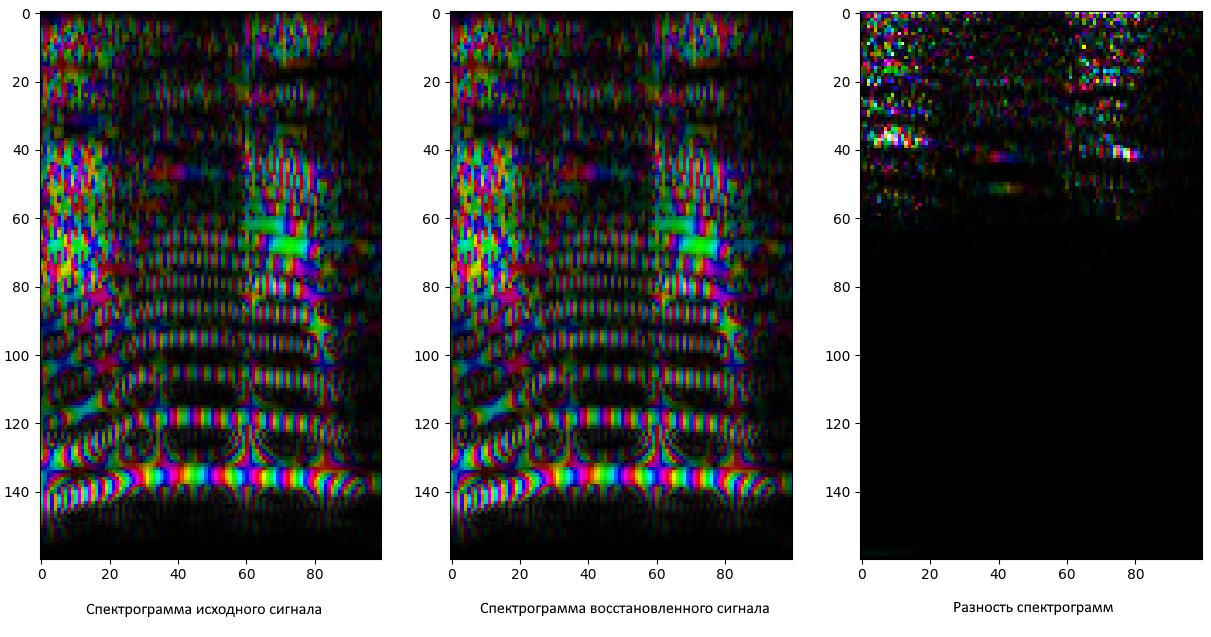
\includegraphics[width=0.8\linewidth]{figures/spec_diff}
  \caption{Спектрограмма сигнала до и после восстановления и их разность}
  \label{fig:spec_diff}
\end{figure}

В случае когда требуется восстановить сигнал максимально точно, необходимо будет выбрать очень маленький шаг свертки.
Маленький шаг свертки ведет к большому количеству точек и большому размеру массива, получаемого в результате преобразования. 
При выборе нелинейной шкалы размеры окон по времени на низких частотах обычно больше шага свертки, что приводит к 
повторению похожих значений в соседних по времени точках, и как следствие к избыточности информации. 
С одной стороны, это повышает устойчивость обратного преобразования к точечным искажениям, 
но с другой стороны приводит к большему потреблению вычислительных ресурсов. 
Иными словами, спектрограмма в нелинейной шкале содержит избыточность информации из-за большего наложения окон в области низких частот.

Если взять за основу мел-шкалу $f(m)$ и ограничить сверху ее производную $df/dm$, 
то в области высоких частот функция $f(m)$ будет переходить из экспоненциальной в линейную, и 
расстояние между соседними частотами $\Delta f_m < \Delta f_{max}$ будет ограничено сверху, 
и можно будет выбрать соответствующий шаг свертки $\Delta t \, \lesssim \, 1 / \Delta f_{max}$. 
Он будет больше, чем для мел-шкалы, что позволит сократить размеры выходного массива, 
при этом сохранив удобную шкалу в области низких и средних частот. 
Если в практическом приложении можно пожертвовать небольшим растяжением области высоких частот, где обычно расположены шумы и шипящие согласные,
то можно использовать такую комбинированную шкалу, чтобы сократить размеры по времени, сохранив восстановимость сигнала.
Пример спектрограммы сигнала до и после восстановления в такой комбинированной шкале и их разность приведены на рисунке \ref{fig:spec_diff_combo_scale}

\begin{figure}
  \centering
  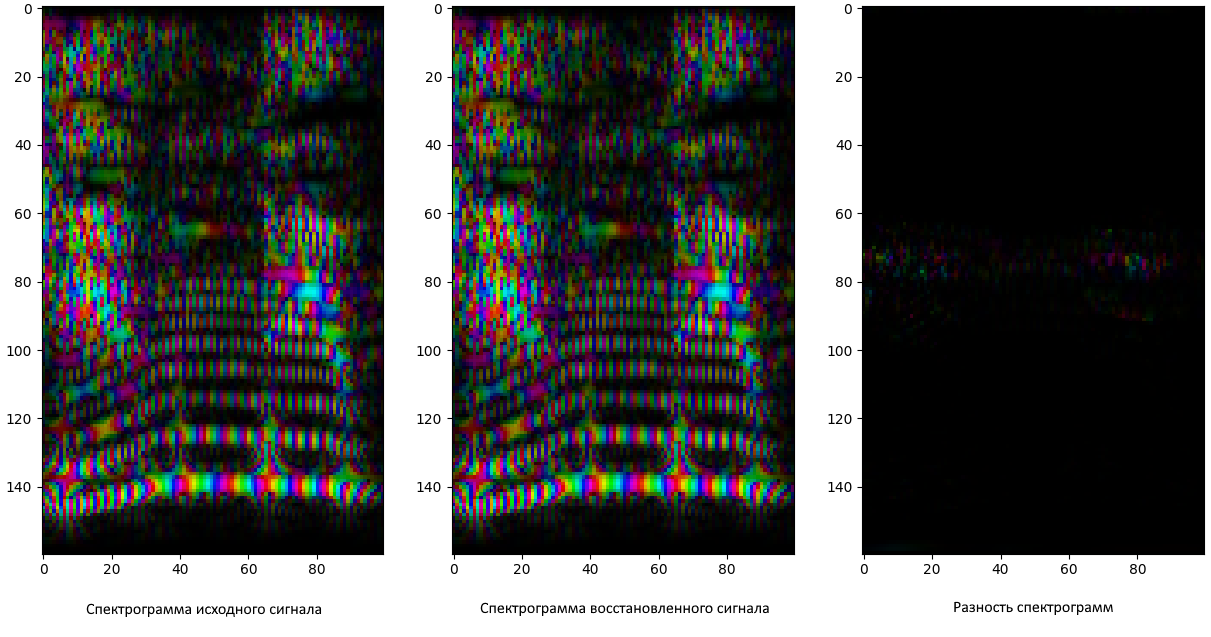
\includegraphics[width=0.8\linewidth]{figures/spec_diff_combo_scale}
  \caption{Спектрограмма сигнала до и после восстановления в комбинированной шкале частот и их разность}
  \label{fig:spec_diff_combo_scale}
\end{figure}


\subsection{Представление фазовой информации в спектрограмме}

Для восстановления сигнала из спектрограммы с помощью описанного выше обратного вейвлет-преобразования, 
в спектрограмме должна быть сохранена фазовая информация (см. Рисунок \ref{fig:complex_spec}). 
Но на практике нейросети для синтеза речи чаще работают со спектрограммами, 
в которых сохранена только магнитудная информация (см. Рисунок \ref{fig:mel_spec}).
Одним из преимуществ формата, где сохранена только магнитуда, является то, что он инвариантен к сдвигу по времени, 
а спектрограмма с сохраненной фазой - не инвариантна. 
Из-за этого нейросети приходится учитывать зависимость фазы от времени, 
что требует дополнительных размерностей признаковых пространств внутри нее.

Чтобы получить спектрограмму с фазовой информацией при помощи нейросети, можно поступить несколькими способами:
\begin{itemize}
  \item Генерировать спектрограмму сразу с фазой - может быть сложно и затратно
  \item Генерировать спектрограмму без фазы, а затем восстановить фазовую информацию. 
    По такому принципу работает декодер на основе алгоритма Гриффина-Лима.
  \item Генерировать спектрограмму, где фазовая часть преобразована обратимым образом.
\end{itemize}

Одним из интересных вариантов обратимого преобразования фазы является взятие производной фазы по времени и вычитание опорной частоты:

\begin{equation}
  \phi(t) = \arg(S_m(t))'_t
\end{equation}
\[ \tilde{S}_m(t) = |S_m(t)|\,e^{i\,\phi(t)}  \, e^{- 2\pi i f_m \Delta t} \]

Пример такого представления изображен на рисунке \ref{fig:freq_diff_repr}

\begin{figure}
  \centering
  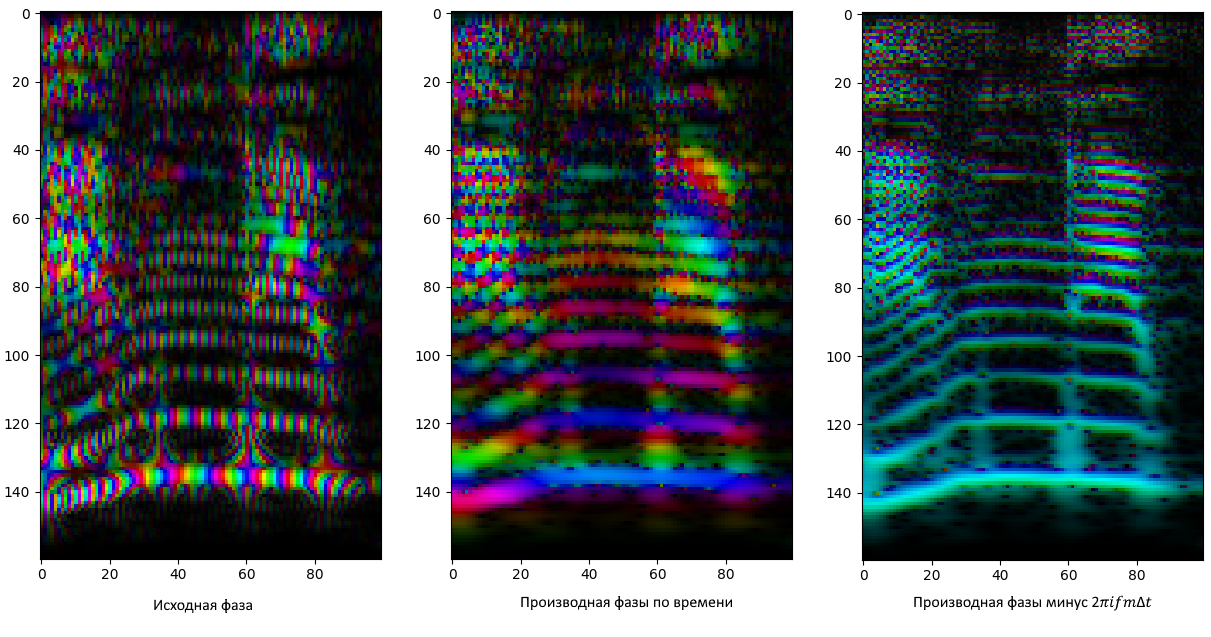
\includegraphics[width=0.8\linewidth]{figures/freq_diff_repr}
  \caption{Представление с производной фазы}
  \label{fig:freq_diff_repr}
\end{figure}

Чтобы восстановить исходную фазу, нужно взять интеграл с переменным верхним пределом от производной фазы, 
и прибавить сохраненное отдельно нулевое значение. К сожалению, такое преобразование неустойчиво к точечным помехам, 
поскольку подразумевает накопление ошибки. Если между соседними частотами фазы немного разойдутся, 
расхождение передастся дальше во времени и будет накапливаться. Поэтому данное преобразование не будет использовано в итоговом алгоритме, 
но такой формат все равно может представлять интерес для задач \textit{распознавания и анализа} речи, или если в будущем удастся найти устойчивое 
обратимое преобразование для получения производной фазы.


\subsection{Алгоритм Гриффина-Лима для вейвлет-преобразования}

Удобным способом получения спектрограммы с фазовой информацией является генерация спектрограммы только с магнитудой, 
и последующее восстановление фазы с помощью специального алгоритма.

В работе были проведены эксперименты, которые показали, что алгоритм Гриффина-Лима (см. раздел \ref{subsubsec:griffinlim})
позволяет восстановить фазовую информацию сигнала, если вместо STFT использовать описанное выше 
вейвлет-преобразование, обобщенное на произвольную шкалу частот (назовем его GWT). В таком случае формулы для итерации алгоритма
будут выглядеть следующим образом:

\begin{equation}
  \tilde{x}_{i+1}(t) = \textbf{IGWT}\{X_i(t, f)\}
  \label{eq:griffin_lim_1}
\end{equation}
\begin{equation}
  \tilde{X}_{i+1} = \textbf{GWT}\{\tilde{x}_{i+1}(t)\}
  \label{eq:griffin_lim_2}
\end{equation}
\begin{equation}
  X_{i+1}(t, f) = X_0(t, f) * e^{i\,\arg(\tilde{X}_{i+1})}
  \label{eq:griffin_lim_3}
\end{equation}

В результате работы алгоритма получается комплекснозначаная спектрограмма с фазовой частью. 
Эксперименты показывают, что она может не совпадать идеально точно с исходной 
из-за незначительных сдвигов во времени некоторых отдельных элементов, но для человека эта разница не слышна.
Качество звука после восстановления сохраняется.

И все же, если нейросеть будет сразу генерировать комплекснозначное представление с фазой, 
качество будет максимальным, а также это позволит избежать вычисления итеративного алгоритма.
Подобный эксперимент был проведен в рамках работы, с его результатами можно ознакомиться в разделе \ref{subsubsec:keep_phase_net}


\section{Реализация алгоритма}

Общая схема прямого и обратного преобразования выглядит следующим образом: (см Рисунок \ref{fig:algorithm_overview})

\clearpage

\begin{figure}
  \centering
  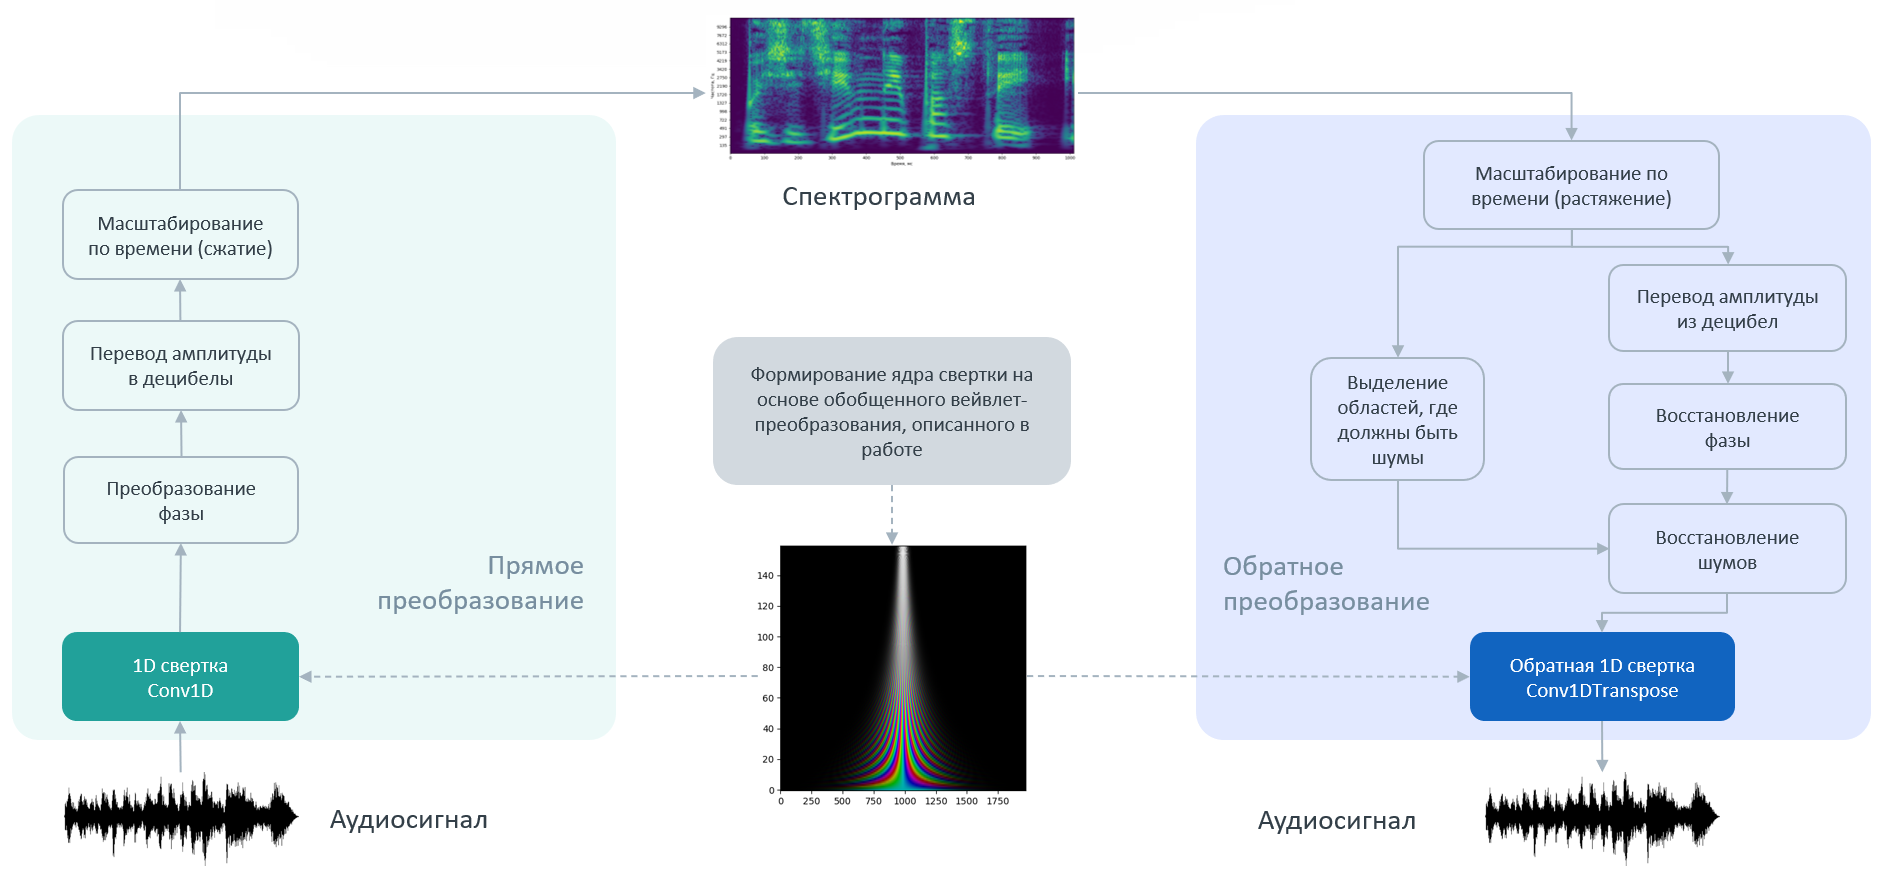
\includegraphics[width=0.9\linewidth]{figures/algorithm_overview}
  \caption{Общая схема прямого и обратного преобразования}
  \label{fig:algorithm_overview}
\end{figure}

\textbf{Прямое преобразование}:
\begin{enumerate}[1.]
  \item 1D свертка с вейвлет-ядром
  \item Преобразование фазы (один из вариантов):
    \begin{itemize}
      \item Сохранение фазы
      \item Отбрасывание фазы, сохранение только магнитуды
    \end{itemize}
  \item (Опционально) Получение энергии из амплитуды смещения
  \item Перевод амплитуды в децибелы
  \item Масштабирование по времени - сжатие
\end{enumerate}

\textbf{Обратное преобразование}:
\begin{enumerate}[1.]
  \item Масштабирование по времени - растяжение
  \item Вычисление маски шумов
  \item Перевод амплитуды в абсолютные значения
  \item (Опционально) Получение амплитуды смещения из энергии
  \item Восстановление фазы (один из вариантов):
    \begin{itemize}
      \item Фаза была сохранена, действие не требуется
      \item Восстановление фазы с помощью адаптированного алгоритма Гриффина-Лима
    \end{itemize}
  \item Обратная 1D свертка с вейвлет-ядром
\end{enumerate}


\subsection{Свертка с вейвлет-ядром}

Рассмотрим поэтапно алгоритм построения вейвлет-спектрограммы с помощью операции свертки Conv1D и восстановления сигнала с помощью
операции Conv1DTranspose.

\textbf{1. Вычисление набора базисных частот} $\{f_m\}$. 
Набор базисных частот вычисляется как набор $M$ равноудаленных точек по мел-шкале в выбранной частотной области.
Количество точек $M$, а также границы частотной области $f_{min}$ и $f_{max}$ задаются как параметр преобразования. 
Обычно $f_{min} = 0$, $f_{max} = f_{discr} / 2$, а $M \in {64 .. 256}$.
Чтобы выбранные точки были равноудалены в мел-шкале, используется следующий алгоритм:
\begin{enumerate}[1.]
  \item Вычисляются мел-значения границ частотной области $\mu_{min} = \mu(f_{min})$, $\mu_{max} = \mu(f_{max})$ по формуле:
  \begin{equation}
    \mu(f) = 1127\,\ln(1 + \frac{f}{700})
  \end{equation}
  
  \item Создается массив $M$ точек между $\mu_{min}$ и $\mu_{max}$, равноудаленных друг от друга:
  \begin{equation}
    \mu_m = \mu_{min} + (\mu_{max} - \mu_{min}) \cdot m / (M - 1), \quad m \in [0, M)
  \end{equation}

  \item Каждая точка в мел-шкале переводится в герцы по формуле:
  \begin{equation}
    f_m = f(\mu_m), \quad f(\mu) = 700 \cdot (e^{\mu / 1127} - 1)
  \end{equation}

  \item Также вычисляются расстояния между соседними частотами $\Delta f_m$:
  \begin{equation}
    \Delta f_m = (f_{m+1} - f_{m-1}) / 2
  \end{equation}
\end{enumerate}

\textbf{2. Формирование ядра свертки}. Происходит в результате выполнения следующих шагов:
\begin{enumerate}[1.]
  \item Определение максимальной ширины окна $N$ и соответственно размера ядра свертки $K: [M \times N]$:
  \begin{equation}
    N = 2 / \min(\Delta f_m)
  \end{equation}

  \item Построение Фурье-базиса из экспонент:
  \begin{equation}
    K_{f}[m, n] = e^{2\pi i f_m (n - N/2) \delta t}, \quad \delta t = 1 / f_d
  \end{equation}

  \item Получение окон для каждой частоты $f_m$ по формуле:
  \begin{equation}
    W[m, n] = w((n - N/2) \delta t \, \Delta f_m)
  \end{equation}

  \item Получение вейвлет-базиса путем умножения экспонент на оконную функцию и нормировочный коэффициент.
  В данной формуле нормировка вейвлетов производится умножением не на $\Delta f_m$ (см. Равенство \ref{eq:psi_wavelet_final}), 
  а на $\sqrt{\Delta f_m}$, чтобы евклидова норма каждого базисного вектора $K_{gwt}[m, ...]$ была одинакова.
  Данное ядро будет использовано для прямого преобразования.
  \begin{equation}
    K_{gwt}[m, n] = K_{f}[m, n] \cdot W[m, n] \cdot \sqrt{\Delta f_m} 
  \end{equation}

  \item Вычисление коэффициента $K_{\psi}[m]$. Для каждой частоты он будет отличаться, поскольку нормировка вейвлетов выполнена по-другому.
  \begin{equation}
    K_{\psi}[m] = \sum \limits_{n = -N S^{-1} / 2}^{N S^{-1} / 2}
      (W [m, N/2 + n \cdot S])^2 , \quad
    S = \Delta t / \delta t
  \end{equation}

  \item Получение ядра для обратного преобразования $\tilde{K}_{gwt}$:
  \begin{equation}
    \tilde{K}_{gwt}[m, n] = K_{gwt}[m, n] \cdot 2 / K_{\psi}[m]
  \end{equation}
\end{enumerate}

\textbf{3. Выполнение свертки для прямого преобразования} происходит с помощью операции Conv1D по формуле:
\begin{equation}
  S[m, n] = \sum \limits_{k=0}^{k=N} x(n\Delta t + k\delta t) \, K_{gwt}[m, k]
\end{equation}

\textbf{4. Выполнение свертки для обратного преобразования} происходит с помощью операции Conv1DTranspose по формуле:
\begin{equation}
  \tilde{x}(n\Delta t + k\delta t) \mathrel{+}= \sum \limits_{m=0}^{m=N} S[m, n] \, \tilde{K}_{gwt}[m, k], \quad 
  \forall k \in [0, N), n \in [0, N_T)
\end{equation}


\subsection{Преобразование фазы}
Предлагается обрабатывать фазовую информацию в спектрограмме следующими способами:

\textbf{1. Передавать без изменений}. В таком случае в нейросеть будет подаваться комплексное представление, 
которое можно разложить либо как действительную и мнимую часть, либо как модуль и фазовый угол.
В таком случае спектрограмма будет не инвариантна к временному сдвигу, что потребует хранить в признаковых пространствах информацию 
о зависимости фазы от времени. Кроме того, шумы с нормальным распределением нейросеть будет сглаживать к среднему значению.
В случае, когда распределение занимает всю комплексную плоскость, это среднее значение будет около нуля. А если бы сохранялась только амплитуда, 
среднее значение было бы пропорционально стандартному отклонению шума.
С другой стороны, для восстановления звука из представления с сохраненной фазой, достаточно выполнить обратную свертку, 
и не требуется выполнение итеративного алгоритма для восстановления фазы.

\textbf{2. Отбрасывать фазу, сохранять только амплитуду}. Этот способ наиболее привычен для популярных нейросетевых моделей. 
Данное представление инвариантно к сдвигу по времени, а также шумы сглаживаются не к нулю, а к значению, 
пропорциональному стандартному отклонению, что позволяет воссоздать другую реализацию шума с такими же параметрами.
После генерации спектрограммы фазовую часть можно восстановить с помощью адаптированного алгоритма Гриффина-Лима.

Адаптированный под вейвлет-преобразование алгоритм Гриффина-Лима выглядит следующим образом:

Пусть исходная спектрограмма с фазовой информацией - $X$, а ее амплитудная часть - $X_0$. 
Также спектрограмма на начальной итерации будет равна $X_i \, |_{i=0} = X_0$, то есть ее действительная часть равна $X_0$, а мнимая равна нулю.
Прямое преобразование на основе свертки - $\textbf{GWT}$, обратное - $\textbf{IGWT}$.
Тогда итерация алгоритма для восстановления фазы:
\begin{equation}
  \tilde{x}_{i+1} = \textbf{IGWT}\{X_{i}\}
\end{equation}
\[\tilde{X}_{i+1} = \textbf{GWT}\{\tilde{x}_{i+1}\}\]
\[X_{i+1} = X_0 \cdot e^{i\, \arg(\tilde{X}_{i+1})}\]

После выполнения некоторого количества итераций (на практике около 60) $X_{i}$ сходится к некоторой спектрограмме 
$\tilde{X}$ с восстановленной фазой, которая по качеству звука не отличается от исходной, слышится человеком точно так же, но отдельные события могут быть незначительно сдвинуты по времени в пределах шага свертки.


\subsection{Преобразование амплитуды}

\textbf{1. Получение энергии колебаний}. Для того, чтобы получить представление, 
в котором амплитуда распределена более равномерно по частотам (см. Рисунок \ref{fig:spectrum_mean}),
амплитуда смещения умножается на частоту: 

\begin{equation}
  S_v[m,n] = S[m,n] \cdot f_m
\end{equation}

Полученное представление пропорционально амплитуде скорости, 
квадрат которой пропорционален энергии колебаний.
Для обратного преобразования амплитуда смещения делится на частоту: 

\begin{equation}
  S[m,n] = S_v[m,n]\,/\,f_m
\end{equation}

\textbf{2. Преобразование в децибелы} относительно порога слышимости $S_0$ производится по формуле:
\begin{equation}
  S_{db} = 20 \cdot \log_{10}(1 + |S_v| / S_0) \cdot e^{i\, \arg(S_v)}
\end{equation}

Обратное преобразование производится по формуле:
\begin{equation}
  S_v = S_0 \cdot (10^{|S_{db}|/20} - 1) \cdot e^{i\, \arg(S_{db})}
\end{equation}


\subsection{Масштабирование}
Для восстановимости сигнала с помощью свертки, должно выполняться ограничение на шаг свертки: $\Delta t < \min(1 / \Delta f_m)$.
Из-за этого может потребоваться избыточное разрешение спектрограммы по времени. 
После отбрасывания фазы можно заметить, что амплитуда меняется не так быстро и можно уменьшить разрешение по времени без потери качества.

Поэтому после отбрасывания фазы можно выполнить сжатие по времени с помощью линейной интерполяции.
Для обратного преобразования выполняется растяжение с помощью линейной интерполяции.


\subsection{Восстановление шумов}

\begin{wrapfigure}{r}{0.25\textwidth}
  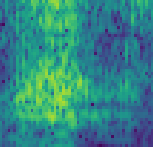
\includegraphics[width=0.9\linewidth]{figures/noise_reconstruction}
  
\includegraphics[width=0.9\linewidth]{figures/noise_reconstruction_smooth}
  \caption{Эффект сглаживания шумов в нейросетях}
  \label{fig:noise_reconstruction}
\end{wrapfigure}

При обучении нейросетей часто используются такие лосс-функции, как средний квардрат ошибки (L2) или средний модуль ошибки (L1), 
или функции, полученные на основе этих. 
Их использование приводит к тому, что модель сначала учится предсказывать крупные объекты и сглаживает шумы к медленно меняющемуся среднему.
Пример такого сглаживания изображен на рисунке \ref{fig:noise_reconstruction}.

В задаче генерации изображений данный эффект не приводит к появлению нежелательных артефактов, а скорее к потере информации. 
Но в задаче генерации звука сглаженные шумы в области высоких частот приводят появлению дребезжащего звука там, 
где он должен быть глухим или шипящим. Этот эффект сильно заметен и нежелателен.

Для того, чтобы синтезировать звук без дребезга при том, что на сгенерированной спектрограмме области шумов сглажены, 
можно прибегнуть к технике восстановления шумов по следующему алгоритму:

\textbf{1. Определение маски шумов}. Для восстановления шума понадобится маска $\alpha[m,n] \in [0, 1]$, 
разделяющая области в частотно-временной плоскости, где представлена либо некоторая реализация шума ($\alpha[m,n] = 1$), 
либо когерентный сигнал ($\alpha[m,n] = 0$) так, как он представлен на спектрограмме без изменений.

Для хорошего качества достаточно сформировать маску по следующему принципу: или частота выше пороговой, где начинается область высоких частот,
обычно занятая шипящими согласными, или амплитуда меньше пороговой, то есть приближается к порогу слышимости и является фоновым шумом.
Математически данное условие можно выразить следующим образом:
\begin{equation}
  \alpha[m,n] = 1 - \sigma\left(\frac{f_t - f_m}{\Delta f_t}\right) \cdot \sigma\left(\frac{S[m,n] - S_t}{\Delta S_t}\right)
\end{equation}

где $f_t$ - пороговая частота, $\Delta f_t$ - ширина полосы перехода частот, $S_t \approx S_0$ - пороговая энергия, 
$\Delta S_t$ - ширина полосы перехода.

\textbf{2. Генерация шума по распределению} и смешение с когерентным сигналом с помощью альфа-маски.
Предполагается, что шум имеет нормальное распределение в исходном комплексном представлении с абсолютными значениями амплитуд.

Сначала генерируется шум с нормальным распределением на множестве комплексных чисел. Среднее значение задается равным нулю.
Стандартное отклонение задается пропорциональным модулю амплитуды на спектрограмме в конкретной точке.
\begin{equation}
  R[m,n] = normal(0,\, S[m,n]) \cdot c
\end{equation}

Затем в комплексном представлении шум смешивается с исходным сигналом по формуле:
\begin{equation}
  S_n[m,n] = R[m,n] \cdot \alpha[m,n] + S[m,n] \cdot (1 - \alpha[m,n])
\end{equation}


\subsection{Визуализация спектрограмм}
При разработке и отладке алгоритма было очень удобно пользоваться функцией визуализации комплекснозначных спектрограмм.
Она преобразует двумерный массив комплексных чисел $S[m,n]$ в RGB-изображение $I[m,n]$, которое может быть отображено на экране или сохранено в файл.

Изображение формируется по следующей формуле:

\begin{equation}
  I[m,n] = \textbf{HSV-to-RGB}\{H[m,n]\}
\end{equation}
\[ H[m,n]_{hue} = \arg(S[m,n]) \]
\[ H[m,n]_{saturation} = \exp(\max(0,\, 1 - \frac{|S[m,n]|}{S_{max}})) \]
\[ H[m,n]_{variance} = \min(1,\, \frac{|S[m,n]|}{S_{max}}) \]


\subsection{Рекомендуемые значения параметров}






\subsection{Предложения для быстрой реализации}


\section{Выводы по главе}
